% ---------------------------------------------------------
% ---- SECTION
% ---------------------------------------------------------
\section{Introduction to the Hybrid Discontinuous Galerkin methods through the Hu-Washizu variational principle}
\label{sec_appendix_composite_demo}

In this section, let $\cell$ a subpart of the body \(\bodyLag\), called a \textit{cell}.
% In the following, one assumes that the
% cell $\cell$ is located inside the body $\bodyLag{}$
% , such that its boundary $\dCell{}$ bears contact loads only.
The cell $\cell$ is in
equilibrium with the rest of the body \(\Omega\backslash T\) if the
displacements and the normal traction are continuous at the boundary
$\dCell{}$.

% ---------------------------------------------------------
% PARAGRAPH
% ---------------------------------------------------------
\paragraph{Conformal methods} Enforcing the displacement continuity at the interface leads to
so-called conformal methods, to which the standard Lagrange Finite Element
method belongs (see Figure \ref{fig_02}(a)).

% ---------------------------------------------------------
% PARAGRAPH
% ---------------------------------------------------------
\paragraph{Discontinuous Galerkin methods} On
the contrary, this condition can be weakened by introducing an elastic
interface of negligible size between \(T\) and \(\Omega\backslash T\).
This representation is at the basis of Discontinuous Galerkin methods
(see Figure \ref{fig_02}(b)).

% ---------------------------------------------------------
% PARAGRAPH
% ---------------------------------------------------------
\paragraph{Hybird Discontinuous Galerkin methods} In
this paper, HDG methods are considered,
where two elastic interfaces are introduced: one between \(T\) and its
boundary \(\partial T\) and a second one between \(\Omega\backslash T\)
and \(\partial T\) (see Figure \ref{fig_02}(c)).
Following this idea,
this section outlines how the use of the Hu-Hashizu Lagrangian allows to
introduce both the
\textit{reconstructed gradient} and the \textit{reconstructed traction force}.

% ---------------------------------------------------------
% -- SUBSECTION
% ---------------------------------------------------------
\subsection{Element description}

% ---------------------------------------------------------
% PARAGRAPH
% ---------------------------------------------------------
\paragraph{Element geometry}

In the following, the cell $\cell$ is assumed to be convex.
It is split into a core part $\Bulk \subset \cell$ with boundary $\dBulk$, and into an interface part $\Crown{} \subset \cell$ with boundary $\dCrown = \dBulk \cup \dCell$, as shown in Figure \ref{fig_02}. The interface $\Crown{}$ has some thickness $\ell > 0$ that is supposed to be small compared to $h_{\cell}$ the diameter of $\cell$.
From a geometrical standpoint, the core part of the element $\Bulk{}$ is an homothety of $\cell$ by some ratio less than $1$.

% ---------------------------------------------------------
% PARAGRAPH
% ---------------------------------------------------------
\paragraph{Element boundary description} The boundary $\dCell{}$ of $\cell$ is the composition of a Neumann boundary $\neumannCell{}$ and a Dirichlet $\dirichletCell{}$, if the element $\cell$ shares a boundary with $\dirichletBoundaryLag{}$. In the following, for the sake of simplicity, the element is assumed to be located inside the body $\bodyLag{}$, such that is only subjected to imposed traction forces on $\neumannCell{} = \dCell{}$ with $\dirichletCell{} = \emptyset$.
%
% 
% 
\begin{figure}[H]
    \centering
    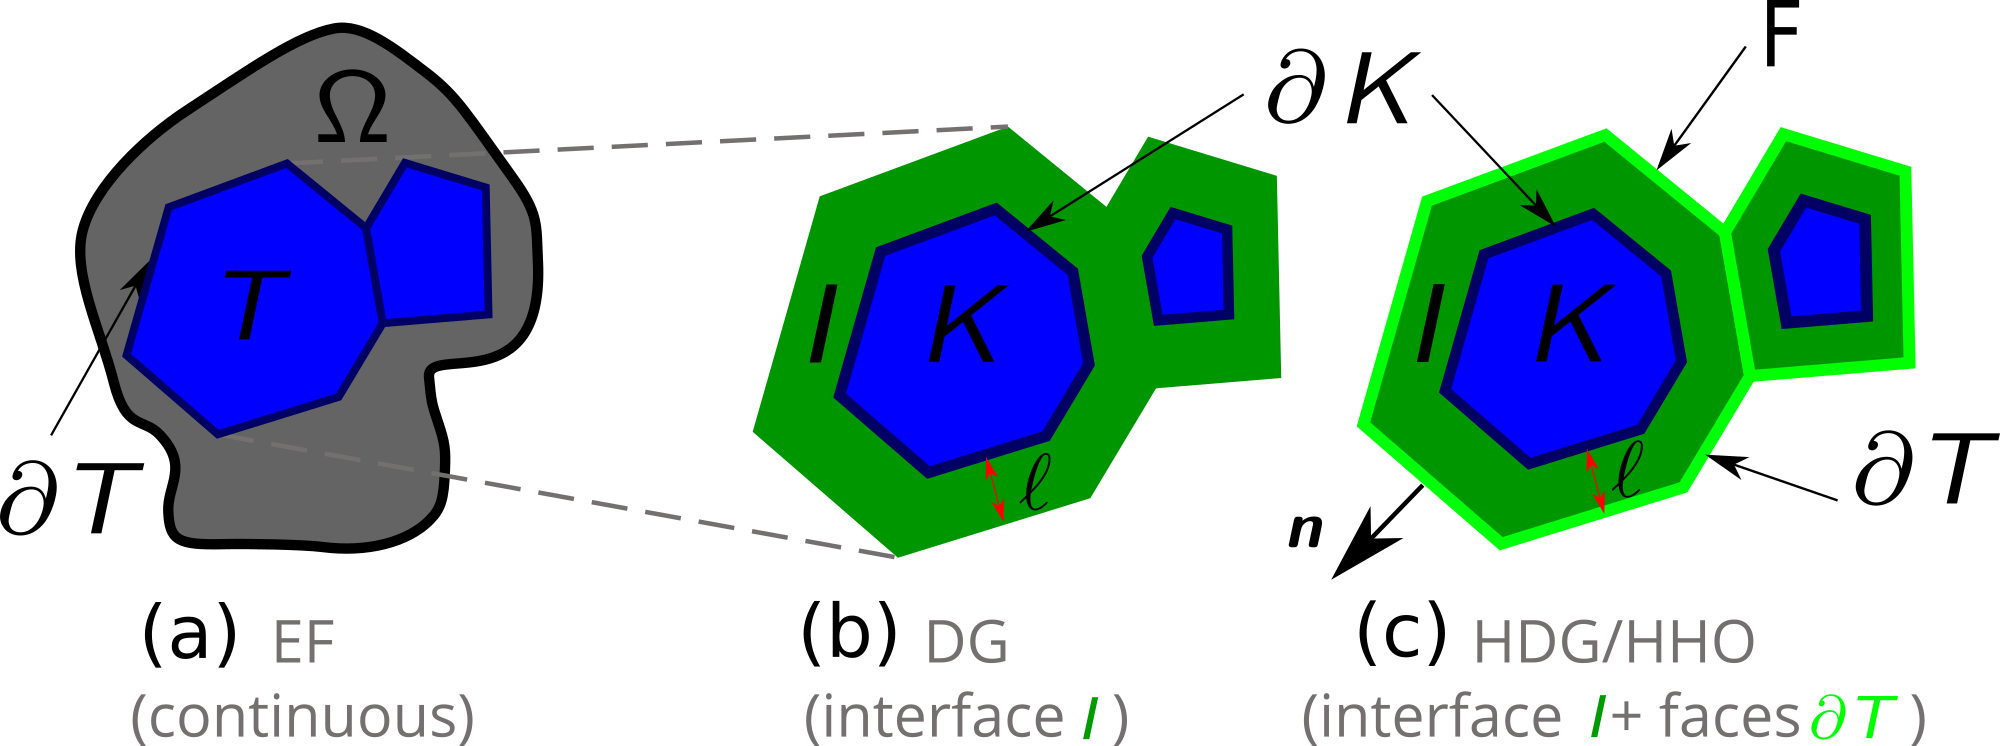
\includegraphics[width=14.cm]{../chapter_002_hho_mechanics/figures/ef_dg_hdg.png}
    \caption{schematic representation of a cell and its surrounding depending on the continuity requirement of the displacement field}
    \label{fig_02}
\end{figure}
%
%
%

% ---------------------------------------------------------
% PARAGRAPH
% ---------------------------------------------------------
\paragraph{Element behaviour}

The core of the element $\Bulk{}$ is made out of the same material that composes $\bodyLag$ and behaves according to the free energy potential $\mecPotential{}_{\bodyLag{}}$. The interface $\Crown{}$ is made out of a pseudo linear elastic material of Young modulus $\beta (\ell / h_{\cell})$ with a zero Poisson ratio and its behavior is defined by the free energy potential $\mecPotential{}_{\Crown{}}$ such that
%
%
%
\begin{equation}
    \label{eq_0009}
        \mecPotential{}_{\Crown} = \frac{1}{2} \beta \frac{\ell}{h_{\cell}} \nabla \tensori{u}{}_{\Crown} : \nabla \tensori{u}{}_{\Crown},
\end{equation}
%
%
%
where the dimensionless ratio $\ell / h_{\cell}$ balances the accumulated energy with the size of the domain $\cell$.

% ---------------------------------------------------------
% PARAGRAPH
% ---------------------------------------------------------
\paragraph{Element loading}

The core $\Bulk$ is subjected to the volumetric loading $\loadLag{}$, and to the traction force applied by the interface $\Crown{}$ onto $\dBulk{}$. By continuity, $\Bulk{}$ applies the opposite traction force on $\Crown{}$ through $\dBulk{}$. The interface $\Crown{}$ is also subjected to the exterior traction force $\neumannCellLoad{}$ acting on $\neumannCell{}$, that accounts for the action of the rest of the solid $\bodyLag{}$ onto the boundary $\dCell$.

% ---------------------------------------------------------
% PARAGRAPH
% ---------------------------------------------------------
\paragraph{Discplacement, displacement gradient and stress fields}

Let note $\tensori{u}{}_{\Bulk}$ the displacement field, $\tensorii{G}{}_{\Bulk}$ the displacement gradient field and $\tensorii{P}{}_{\Bulk}$ the stress field in $\Bulk{}$. Similarly, let $\tensori{u}{}_{\Crown{}}$ the displacement field, $\tensorii{G}{}_{\Crown}$ the displacement gradient field and $\tensorii{P}{}_{\Crown}$ the stress field in $\Crown{}$.
The displacement of the boundary $\dCell{}$ is denoted $\tensori{u}{}_{\dCell{}}$.
By continuity of the displacement field between $\Bulk{}$ and $\dCell$,  the displacement $\tensori{u}{}_{\Crown{}}$ verifies
%
% 
% 
\begin{subequations}
    \label{eq_conformity}
        \begin{alignat}{2}
        \tensori{u}{}_{\Crown} \vert_{\dBulk} & = \tensori{u}{}_{\Bulk} \vert_{\dBulk}
        \label{eq_conformity:eq1},
        \\
        \tensori{u}{}_{\Crown} \vert_{\dCell} & = \tensori{u}{}_{\dCell}
        \label{eq_conformity:eq2}.
    \end{alignat}
\end{subequations}

% ---------------------------------------------------------
% PARAGRAPH
% ---------------------------------------------------------
\paragraph{Hu-Washizu Lagrangian of the element}

By combining both the Lagragian of the core $\Bulk{}$ and that of the interface $\Crown{}$, one obtains the total Lagragian $L_{\cell}^{HW}$ over the element such that
%
%
%
\begin{equation}
    \label{eq_hu_washizu_split}
    L_{\cell}^{HW}
    % (\tensori{u}{}_{\cell}, \tensorii{G}{}_{\cell}, \tensorii{P}{}_{\cell})
    =
    \int_{\Bulk} \mecPotential_{\bodyLag{}} + \int_{\Bulk} (\nabla \tensori{u}{}_{\Bulk} - \tensorii{G}{}_{\Bulk}) : \tensorii{P}{}_{\Bulk}
    +
    \int_{\Crown} \mecPotential_{\Crown{}} + \int_{\Crown} (\nabla \tensori{u}{}_{\Crown} - \tensorii{G}{}_{\Crown}) : \tensorii{P}{}_{\Crown}
    -
    \int_{\Bulk} \loadLag \cdot \tensori{u}{}_{\Bulk}
    % -
    % \int_{\Crown} \loadLag \cdot \tensori{u}{}_{\Crown}
    -
    \int_{\neumannCell} \neumannCellLoad \cdot \tensori{u}{}_{\dCell},
\end{equation}

% ---------------------------------------------------------
% -- SUBSECTION
% ---------------------------------------------------------
\subsection{Hypotheses}
\label{sec_assumtions}

% Since the interface is of negligible volume compared to that of the core, the following assumptions are made on the displacement and the stress fields in the interface:

% ---------------------------------------------------------
% PARAGRAPH
% ---------------------------------------------------------
\paragraph{Displacement in the interface}

Since the interface is of negligible volume compared to that of the core, the displacement in the interface $\Crown$ is assumed to be linear with respect to $\tensori{n}$, such that
its gradient is homogeneous in $\Crown{}$ along $\tensori{n}$
%
% 
% 
\begin{equation}
    \label{eq_crown_displacement}
    \nabla
    \tensori{u}{}_{\Crown}
    =
    \frac{\tensori{u}{}_{\dCell}
    -
    \tensori{u}{}_{\Bulk} \vert_{\dBulk} }{\ell} \otimes \tensori{n}.
\end{equation}
% 
% 
%
That is, the displacement of the interface $\Crown{}$ linearly bridges that of the boundary $\dCell{}$ to that of the bulk $\Bulk{}$.

% ---------------------------------------------------------
% PARAGRAPH
% ---------------------------------------------------------
\paragraph{Stress in the interface}

Likewise, let assume that $\tensorii{P}{}_{\Crown}$ is constant along the direction $\tensori{n}{}$ in $\Crown{}$. By continuity of the traction force across $\dBulk$, the following equality holds true
%
% 
% 
\begin{equation}
    \label{eq_continuity_traction_force}
    \begin{aligned}
        (\tensorii{P}{}_{\Crown} - \tensorii{P}{}_{\Bulk} \vert_{\dBulk{}}) \cdot \tensori{n}{} = 0
        &&
        \text{on}
        &&
        \dBulk{}.
        % &&
        % \text{in}
        % &&
        % \Crown{}
    \end{aligned}
\end{equation}

% ---------------------------------------------------------
% -- SUBSECTION
% ---------------------------------------------------------
\subsection{Towards Hybrid discontinuous methods from the Hu-Washizu Lagrangian}

% Using the hypotheses stated in Section \ref{sec_assumtions} on the displacement and the stress field in $\Crown{}$,
% \eqref{eq_hu_washizu_split} can be expressed as a term depending on the thickness of the interface $\ell$ and on the core and boundary unknowns only.
% In particular, making the thickness of the interface $\ell \rightarrow 0$, such that $\Crown{}$ vanishes and the core part $\Bulk{}$ identifies to $\cell$,
% a simplified expression of \eqref{eq_hu_washizu_split} is obtained.
% The reader can refer to \ref{sec_appendix_Hu_Washizu} for more details on technical details.

% ---------------------------------------------------------
% PARAGRAPH
% ---------------------------------------------------------
\paragraph{Simplified Hu–Washizu Lagrangian for a vanishing interface}

% In particular, making the thickness of the interface $\ell \rightarrow 0$, such that $\Crown{}$ vanishes and the core part $\Bulk{}$ identifies to $\cell$,
% The following simplified Hu–Washizu Lagrangian is obtained (See \ref{sec_appendix_Hu_Washizu})
% Using hypotheses expressed in Section \ref{sec_assumtions} and making $\ell \rightarrow 0$, the following simplified Hu–Washizu Lagrangian arises from \eqref{eq_hu_washizu_split}
Using the hypotheses stated in Section \ref{sec_assumtions} on the displacement and the stress field in $\Crown{}$,
\eqref{eq_hu_washizu_split} can be expressed as a term depending on the thickness of the interface $\ell$ and on the core and boundary unknowns only.
In particular, making the thickness of the interface $\ell \rightarrow 0$, such that $\Crown{}$ vanishes and the core part $\Bulk{}$ identifies to $\cell$,
a simplified expression of \eqref{eq_hu_washizu_split} is obtained
% 
% 
%
\begin{equation}
    \label{eq_0015}
    \begin{aligned}
        L_{\cell}^{HW}
        = &
        \int_{\cell{}} \mecPotential{}_{\bodyLag{}} + \int_{\cell{}} (\nabla \tensori{u}{}_{\cell{}} - \tensorii{G}{}_{\cell{}}) : \tensorii{P}{}_{\cell}
        % \\
        % &
        + \int_{\dCell{}} (\tensori{u}{}_{\dCell} - \tensori{u}{}_{\cell} \vert_{\dCell}) \cdot \tensorii{P}{}_{\cell} \vert_{\dCell{}} \cdot \tensori{n}{}
        % \\
        % &
        + \int_{\dCell} \frac{\beta}{2 h_{\cell}} \lVert \tensori{u}{}_{\dCell{}} - \tensori{u}{}_{\cell{}} \vert_{\dCell{}} \rVert^2
        \\
        &
        -
        \int_{\cell} \loadLag{} \cdot \tensori{u}{}_{\cell{}}
        -
        \int_{\neumannCell{}} \neumannCellLoad{} \cdot \tensori{u}{}_{\dCell{}},
    \end{aligned}
\end{equation}
%
%
%
such that \eqref{eq_0015} fully defines the equilibrium of an element in the context of hybrid discontinuous methods. The reader can refer to \ref{sec_appendix_Hu_Washizu} for more details on technical details.

% ---------------------------------------------------------
% PARAGRAPH
% ---------------------------------------------------------
\paragraph{HDG methods and hybridization of the primal unknown}

Since the interface $\Crown{}$ has vanished, both $\tensori{u}{}_{\cell} \vert_{\dCell{}}$ the trace of the displacement of the core part $\cell$ onto $\dCell{}$ and $\tensori{u}{}_{\dCell{}}$ the displacement of the boundary coexist on $\dCell{}$. The displacement of the element $\cell$ is thus said to be \textit{hybrid}, and is denoted by the pair $(\tensori{u}{}_{\cell}, \tensori{u}{}_{\dCell})$.

% ---------------------------------------------------------
% PARAGRAPH
% ---------------------------------------------------------
\paragraph{The special case of DG methods}

Replacing $\tensori{u}{}_{\dCell}$ by $\tensori{u}{}_{\cell'} \vert_{\dCell}$ for any neighboring cell $\cell'$ amounts to describe the framework of Discontinuous Galerkin methods, where only the core unknown $\tensori{u}{}_{\cell}$ is considered, and the displacement jump on $\dCell$ depends on $\tensori{u}{}_{\cell'} \vert_{\dCell}$ the trace of the displacement of neighboring cells instead.

% ---------------------------------------------------------
% PARAGRAPH
% ---------------------------------------------------------
\paragraph{Conformal Galerkin formulation}

By strongly enforcing continuity of the displacement across $\dCell{}$ such that $\tensori{u}_{\cell} \vert_{\dCell} = \tensori{u}_{\dCell}$, one recovers the Principle of Virtual Work \eqref{eq_HW_0}, which defines the framework of conformal methods.

% ---------------------------------------------------------
% PARAGRAPH
% ---------------------------------------------------------
\paragraph{Lagrangian variations}

By differentiation of the total Lagrangian \eqref{eq_0015} with respect to each variable of the problem, the following weak equations arise
%
%
%
\begin{subequations}
    \label{eq_0017}
        \begin{alignat}{3}
            \langle \frac{\partial L_{\cell}^{HW}}{\partial \tensori{u}{}_{\cell}} , \delta \tensori{u}{}_{\cell} \rangle
            = & \int_{\cell} \tensorii{P}{}_{\cell} : \nabla \delta \tensori{u}{}_{\cell}
            -
            \int_{\cell} \tensori{f}{}_V \cdot \delta \tensori{u}{}_{\cell}
            -
            \int_{\dCell{}} \tensori{\theta}{}_{\cell} \cdot \delta \tensori{u}{}_{\cell} \vert_{\dCell}
            &&
            \ \ \ \ \ \ \ \ 
            &&
            \forall \delta \tensori{u}{}_{\cell},
            % \in \virtualDisplacementSpaceCell
        \label{eq_0017:eq0}
        \\
            \langle \frac{\partial L_{\cell}^{HW}}{\partial \tensori{u}{}_{\dCell}} , \delta \tensori{u}{}_{\dCell} \rangle
            = &
            \int_{\neumannCell} (\tensori{\theta}{}_{\cell} - \tensori{t}{}_{\neumannCell}) \cdot \delta \tensori{u}{}_{\dCell}
            &&
            \ \ \ \ \ \ \ \ 
            &&
            \forall \delta \tensori{u}{}_{\dCell},
            % \in \virtualDisplacementSpaceDCell
        \label{eq_0017:eq1}
        \\
            \langle \frac{\partial L_{\cell}^{HW}}{\partial \tensorii{P}{}_{\cell}} , \delta \tensorii{P}{}_{\cell} \rangle
            = & \int_{\cell} (\nabla \tensori{u}{}_{\cell} - \tensorii{G}{}_{\cell} ) : \delta \tensorii{P}{}_{\cell}
            +
            \int_{\dCell} (\tensori{u}{}_{\dCell} - \tensori{u}{}_{\cell} \vert_{\dCell}) \cdot \delta \tensorii{P}{}_{\cell} \vert_{\dCell} \cdot \tensori{n}{}
            &&
            \ \ \ \ \ \ \ \ 
            &&
            \forall \delta \tensorii{P}{}_{\cell},
            % \in \stressSpaceCell
        \label{eq_0017:eq3}
        \\
            \langle \frac{\partial L_{\cell}^{HW}}{\partial \tensorii{G}{}_{\cell}} , \delta \tensorii{G}{}_{\cell} \rangle
            = &
            \int_{\cell} (\frac{\partial \mecPotential_{\bodyLag}}{\partial \tensorii{G}{}_{\cell}} - \tensorii{P}{}_{\cell}) : \delta \tensorii{G}{}_{\cell}
            &&
            \ \ \ \ \ \ \ \ 
            &&
            \forall \delta \tensorii{G}{}_{\cell},
            % \in \gradSpaceCell
        \label{eq_0017:eq2}
    \end{alignat}
\end{subequations}
% 
% 
%
where the \textit{reconstructed traction force} $\tensori{\theta}{}_{\cell} = \tensorii{P}{}_{\cell} \vert_{\dCell} \cdot \tensori{n}{} + (\beta / h_{\cell}) \tensori{J}(\tensori{u}{}_{\cell}, \tensori{u}{}_{\dCell})$ is introduced, with
$\tensori{J}(\tensori{u}{}_{\cell}, \tensori{u}{}_{\dCell}) = \tensori{u}{}_{\dCell} - \tensori{u}{}_{\cell} \vert_{\dCell}$ the jump function on the boundary $\dCell$.
Following discretization, multiple jump function choices are available. The reader can refer to \ref{sec_stabilization} for more details regarding implementation aspects.
In particular, \eqref{eq_0017:eq0} is the expression of the Principle of Virtual Work in $\cell$, where the \textit{reconstructed traction force} $\tensori{\theta}{}_{\cell}$ replaces the usual expression $\tensorii{P}{}_{\cell} \cdot \tensori{n}{}$ in the external contribution. \eqref{eq_0017:eq1} denotes a supplementary equation to the usual continuous problem as described in \eqref{eq_hu_washizu_derivative_0}, to account for the continuity of the flux $\tensori{\theta}{}_{\cell}$ across the cell boundary.
\eqref{eq_0017:eq2} accounts for the constitutive equation in a weak sense, and \eqref{eq_0017:eq3} defines the equation of an enhanced gradient field, that does not reduce to the projection of $\nabla \tensori{u}{}_{\cell}$ as in \eqref{eq_hu_washizu_derivative_0:eq3}, since it is enriched by a boundary component that depends on the displacement jump.
This feature is at the origin of the robustness of non-conformal methods to volumetric locking (see \ref{sec_appendix_gradient} for more details on this note).

% ---------------------------------------------------------
% -- SUBSECTION
% ---------------------------------------------------------
\subsection{Problem in primal form}
\label{sec_hdg_element_equilibrium}

% ---------------------------------------------------------
% PARAGRAPH
% ---------------------------------------------------------
\paragraph{Reconstructed gradient}

Since minimization of \eqref{eq_0017:eq3} defines a linear problem with any displacement pair $(\tensori{v}{}_{\cell}, \tensori{v}{}_{\dCell})$, one can eliminate \eqref{eq_0017:eq3} from the system \eqref{eq_0017}. The resulting equation defines the so-called \textit{reconstructed gradient} $\tensorii{G}{}_{\cell}(\tensori{v}{}_{\cell}, \tensori{v}{}_{\dCell})$ associated with any displacement pair $(\tensori{v}{}_{\cell}, \tensori{v}{}_{\dCell})$, that satisfies
%
%
%
\begin{equation}
    \label{eq_grad}
    \begin{aligned}
        \int_{\cell} \tensorii{G}{}_{\cell} : \tensorii{\tau}{}_{\cell}
        =
        \int_{\cell}  \nabla \tensori{v}{}_{\cell} : \tensorii{\tau}{}_{\cell}
        +
        \int_{\dCell} (\tensori{v}{}_{\dCell} - \tensori{v}{}_{\cell} \vert_{\dCell}) \cdot \tensorii{\tau}{}_{\cell} \vert_{\dCell} \cdot \tensori{n}{}
        &&
        \forall \tensorii{\tau}{}_{\cell},
        % \in \stressSpaceCell
    \end{aligned}
\end{equation}
%
%
%
where $\tensorii{\tau}{}_{\cell}$ denotes an arbitrary kinematically admissible stress field.

% -> expliquer que quand saut tend vers 0, on retrouve le projection normale
%  ordre du gradient -> dire que même ordre que approximation primale, renvoie aux annexes

% ---------------------------------------------------------
% PARAGRAPH
% ---------------------------------------------------------
\paragraph{Stress tensor}

Likewise, \eqref{eq_0017:eq2} is eliminated from \eqref{eq_0017} since it is linear with $\tensorii{G}{}_{\cell}$. Assuming in addition that the space of kinematically admissible stress fields is included in that of kinematically admissible displacement gradient fields, \eqref{eq_0017:eq2} holds in a strong sense such that
%
%
%
\begin{equation}
    \label{eq_stress}
    \begin{aligned}
        \tensorii{P}{}_{\cell} = \frac{\partial \mecPotential_{\bodyLag}}{\partial \tensorii{G}{}_{\cell}}.
    \end{aligned}
\end{equation}

% ---------------------------------------------------------
% PARAGRAPH
% ---------------------------------------------------------
\paragraph{Lagrangian variations in primal form}

Using \eqref{eq_stress} and \eqref{eq_grad}, problem \eqref{eq_0017} depends on the displacement unknowns only.
% and the only remaining variations of the total Lagrangian \eqref{eq_0015} are those with respect to both displacement variables.
A new total Lagrangian $L_{\cell}^{HDG}$ arises from the simplified problem such that
%
%
%
\begin{equation}
    \label{eq_total_lagragian_bis}
    \begin{aligned}
        L_{\cell}^{HDG}
        = &
        \int_{\cell{}} \mecPotential_{\bodyLag}
        +
        \int_{\dCell} \frac{\beta}{2 h_{\cell}} \lVert \tensori{J}(\tensori{u}{}_{\cell{}}, \tensori{u}{}_{\dCell{}}) \rVert^2
        -
        \int_{\cell} \loadLag{} \cdot \tensori{u}{}_{\cell{}}
        -
        \int_{\neumannCell{}} \neumannCellLoad{} \cdot \tensori{u}{}_{\dCell{}},
    \end{aligned}
\end{equation}
%
%
%
with respective cell and boundary displacement variations:
\begin{subequations}
    \label{eq_final_problem}
        \begin{alignat}{3}
            \langle \frac{\partial L_{\cell}^{HDG}}{\partial \tensori{u}{}_{\cell}} , \delta \tensori{u}{}_{\cell} \rangle
            = & \int_{\cell} \tensorii{P}{}_{\cell} : \nabla \delta \tensori{u}{}_{\cell}
            -
            \int_{\cell} \tensori{f}{}_V \cdot \delta \tensori{u}{}_{\cell}
            -
            \int_{\dCell{}} \tensori{\theta}{}_{\cell} \cdot \delta \tensori{u}{}_{\cell} \vert_{\dCell}
            &&
            \qquad
            &&
            \forall \delta \tensori{u}{}_{\cell},
            % \in \virtualDisplacementSpaceCell
        \label{eq_final_problem:eq0}
        \\
            \langle \frac{\partial L_{\cell}^{HDG}}{\partial \tensori{u}{}_{\dCell}} , \delta \tensori{u}{}_{\dCell} \rangle
            = &
            \int_{\neumannCell} (\tensori{\theta}{}_{\cell} - \tensori{t}{}_{\neumannCell}) \cdot \delta \tensori{u}{}_{\dCell}
            &&
            \qquad
            &&
            \forall \delta \tensori{u}{}_{\dCell},
        \label{eq_final_problem:eq1}
    \end{alignat}
\end{subequations}
%
%
%
where $\tensorii{P}{}_{\cell}$ is defined by \eqref{eq_stress} and
depends on $\tensorii{G}{}_{\cell}$ which solves \eqref{eq_grad}.

\subsection{Restriction to the Small strain hypothesis}

The proposed large deformation formulation also allows for a natural transition to the small deformation framework. In this context, the gradient of the transformation $\tensorii{F}{}_{\cell}$ is assumed to be small compared to the identity $\tensorii{I}$, and the infinitesimal deformation field $\tensorii{\varepsilon}_{\cell}$ is sought in place of $\tensorii{F}{}_{\cell}$ such that
% \eqref{eq_grad_def} writes
%
%
%
\begin{equation}
    \tensorii{\varepsilon}{}_{\cell} - \nabla^s \tensori{u}{}_{\cell} = 0,
\end{equation}
%
%
%
where the symmetric displacement gradient $\nabla^s \tensori{u}{}_{\cell}$ replaces 
the usual displacement gradient in \eqref{eq_grad_def}.
The stress tensor $\tensorii{P}{}_{\cell}$ is then identified with the Cauchy stress $\tensorii{\sigma}{}_{\cell}$, such that the Lagrangian \eqref{eq_0015} becomes
%
%
%
\begin{equation}
    \label{eq_small_defs}
    \begin{aligned}
        L_{\cell}^{HW}
        = &
        \int_{\cell{}} \mecPotential{}_{\bodyLag{}} + (\nabla^s \tensori{u}{}_{\cell{}} - \tensorii{\varepsilon}{}_{\cell{}}) : \tensorii{\sigma}{}_{\cell}
        % \\
        % &
        + \int_{\dCell{}} (\tensori{u}{}_{\dCell} - \tensori{u}{}_{\cell} \vert_{\dCell}) \cdot \tensorii{\sigma}{}_{\cell} \vert_{\dCell{}} \cdot \tensori{n}{}
        % \\
        % &
        + \int_{\dCell} \frac{\beta}{2 h_{\cell}} \lVert \tensori{u}{}_{\dCell{}} - \tensori{u}{}_{\cell{}} \vert_{\dCell{}} \rVert^2
        \\
        &
        -
        \int_{\cell} \loadLag{} \cdot \tensori{u}{}_{\cell{}}
        -
        \int_{\neumannCell{}} \neumannCellLoad{} \cdot \tensori{u}{}_{\dCell{}},
    \end{aligned}
\end{equation}
%
%
%
where for any pair $(\tensori{v}{}_{\cell}, \tensori{v}{}_{\dCell})$ the \textit{reconstructed strain} $\tensorii{\varepsilon}{}_{\cell}(\tensori{v}{}_{\cell}, \tensori{v}{}_{\dCell})$ is evaluated against any kinematically admissible symmetric stress field $\tensorii{\tau}{}_{\cell}$ such that
%
%
%
\begin{equation}
    \label{eq_grad_ss}
    \begin{aligned}
        \int_{\cell} \tensorii{\varepsilon}{}_{\cell} : \tensorii{\tau}{}_{\cell}
        =
        \int_{\cell}  \nabla^s \tensori{v}{}_{\cell} : \tensorii{\tau}{}_{\cell}
        +
        \int_{\dCell} (\tensori{v}{}_{\dCell} - \tensori{v}{}_{\cell} \vert_{\dCell}) \cdot \tensorii{\tau}{}_{\cell} \vert_{\dCell} \cdot \tensori{n}{}
        &&
        \forall \tensorii{\tau}{}_{\cell},
        % \in \stressSpaceCell
    \end{aligned}
\end{equation}
%
%
%
and the Cauchy stress is the derivative of the potential $\mecPotential_{\bodyLag{}}$ with respect to $\tensorii{\varepsilon}{}_{\cell}$
%
%
%
\begin{equation}
    \label{eq_stress_ss}
    \begin{aligned}
        \tensorii{\sigma}{}_{\cell} = \frac{\partial \mecPotential_{\bodyLag}}{\partial \tensorii{\varepsilon}{}_{\cell}}.
    \end{aligned}
\end{equation}

% \subsection{Extension to the axi-symmetric framework}

% In the following section, we devise a Hybrid High order method for an axi-symmetric framework. Owing to geometrical assumptions on the displacement and its gradient, the definition of the reconstructed gradient \eqref{eq_grad} and of that of the higher order displacement \eqref{eq_potential} needs be modified accordingly. Details about the definitions of these ingredients can be found in \ref{sec_appendix_axi}.

% \paragraph{Axi-symmetric framework}

% The cartesian space is expressed in cylindrical coordinates and a point $\tensori{X} \in \bodyLag$ has coordinates $\tensori{X} = (r, z, \theta)$ where $r$ denotes the radial component, $z$ the ordinate one, and $\theta$ is the angular component describing a revolution around the axis $r = 0$. By cylindrical symmetry, the angular displacement $\tensoro{u}{}_{\theta}$ is supposed to be zero, and both components $u_r$ and $u_z$ do not depend on the angular coordinate $\theta$.

% % \paragraph{Cell displacement gradient}

% % % Adopting notations introduced in Section \ref{sec_composite_demo}, let $\cell$ an open subset of $\bodyLag \subset \mathbb{R}^2$ in the $(r,z)$ plane with cell displacement $\tensori{u}{}_{\cell} \in \displacementSpaceCell$ and boundary displacement $\tensori{u}{}_{\dCell} \in \displacementSpaceDCell$.
% % The partial derivatives of $\tensori{u}{}_{\cell}$ with respect to the cylindrical coordinates are given by
% % %
% % %
% % %
% % \begin{equation}
% %     \begin{aligned}
% %         \forall i, j \in \{ r,z \}, \tensoro{u}{}_{\cell i,j} = \frac{\partial u_{\cell i}}{\partial j} && \text{and} && \tensoro{u}{}_{\cell \theta, \theta} = \frac{u_{\cell r}}{r}
% %     \end{aligned}
% % \end{equation}

% \paragraph{Axis faces treatment}

% Since in cylindrical coordinates, all integrals depend on the radial component $r$, boundary integrals vanish at $r = 0$ on the symmetry axis.
% Therefore, the reconstructed gradient (and the stabilization) do not depend on a closed surface wrapping a cell $\cell$ located on the symmetry axis.
% However, this feature is necessary to prove the robustness of the HHO method to volumetric locking (see \ref{sec_appendix_gradient}).
% Therefore, in order to restore full mobility of a face located on the symmetry axis, we consider infinitely thin cylindrical faces wrapping it, that are subjected to Dirichlet boundary conditions along the radial direction.

